\documentclass[12pt, a4paper]{article}
\usepackage[spanish]{babel}
\usepackage[utf8]{inputenc}
\usepackage{graphicx}
\usepackage{geometry}
\usepackage{fancyhdr}
\usepackage{float}

\geometry{a4paper, margin=2.5cm}
\pagestyle{fancy}
\fancyhf{}
\rhead{Informe Tecnología en la Vida Cotidiana}
\lhead{Grupo XX}
\rfoot{Página \thepage}

\title{Informe: Tecnología en la Vida Cotidiana}
\author{Nombre del Integrante}
\date{\today}

\begin{document}

\maketitle

\section*{Criterios de Selección}
\begin{itemize}
    \item Criterio 1: Relevancia en el impacto tecnológico actual
    \item Criterio 2: Disponibilidad de datos actualizados
    \item Criterio 3: Representatividad sectorial
    \item Criterio 4: Capacidad de visualización comparativa
\end{itemize}

\section*{Análisis Gráfico}

% Repite este bloque para cada gráfico (total 6)
\subsection*{Gráfico 1: Aquí colocar título}
\begin{figure}[H]
    \centering
    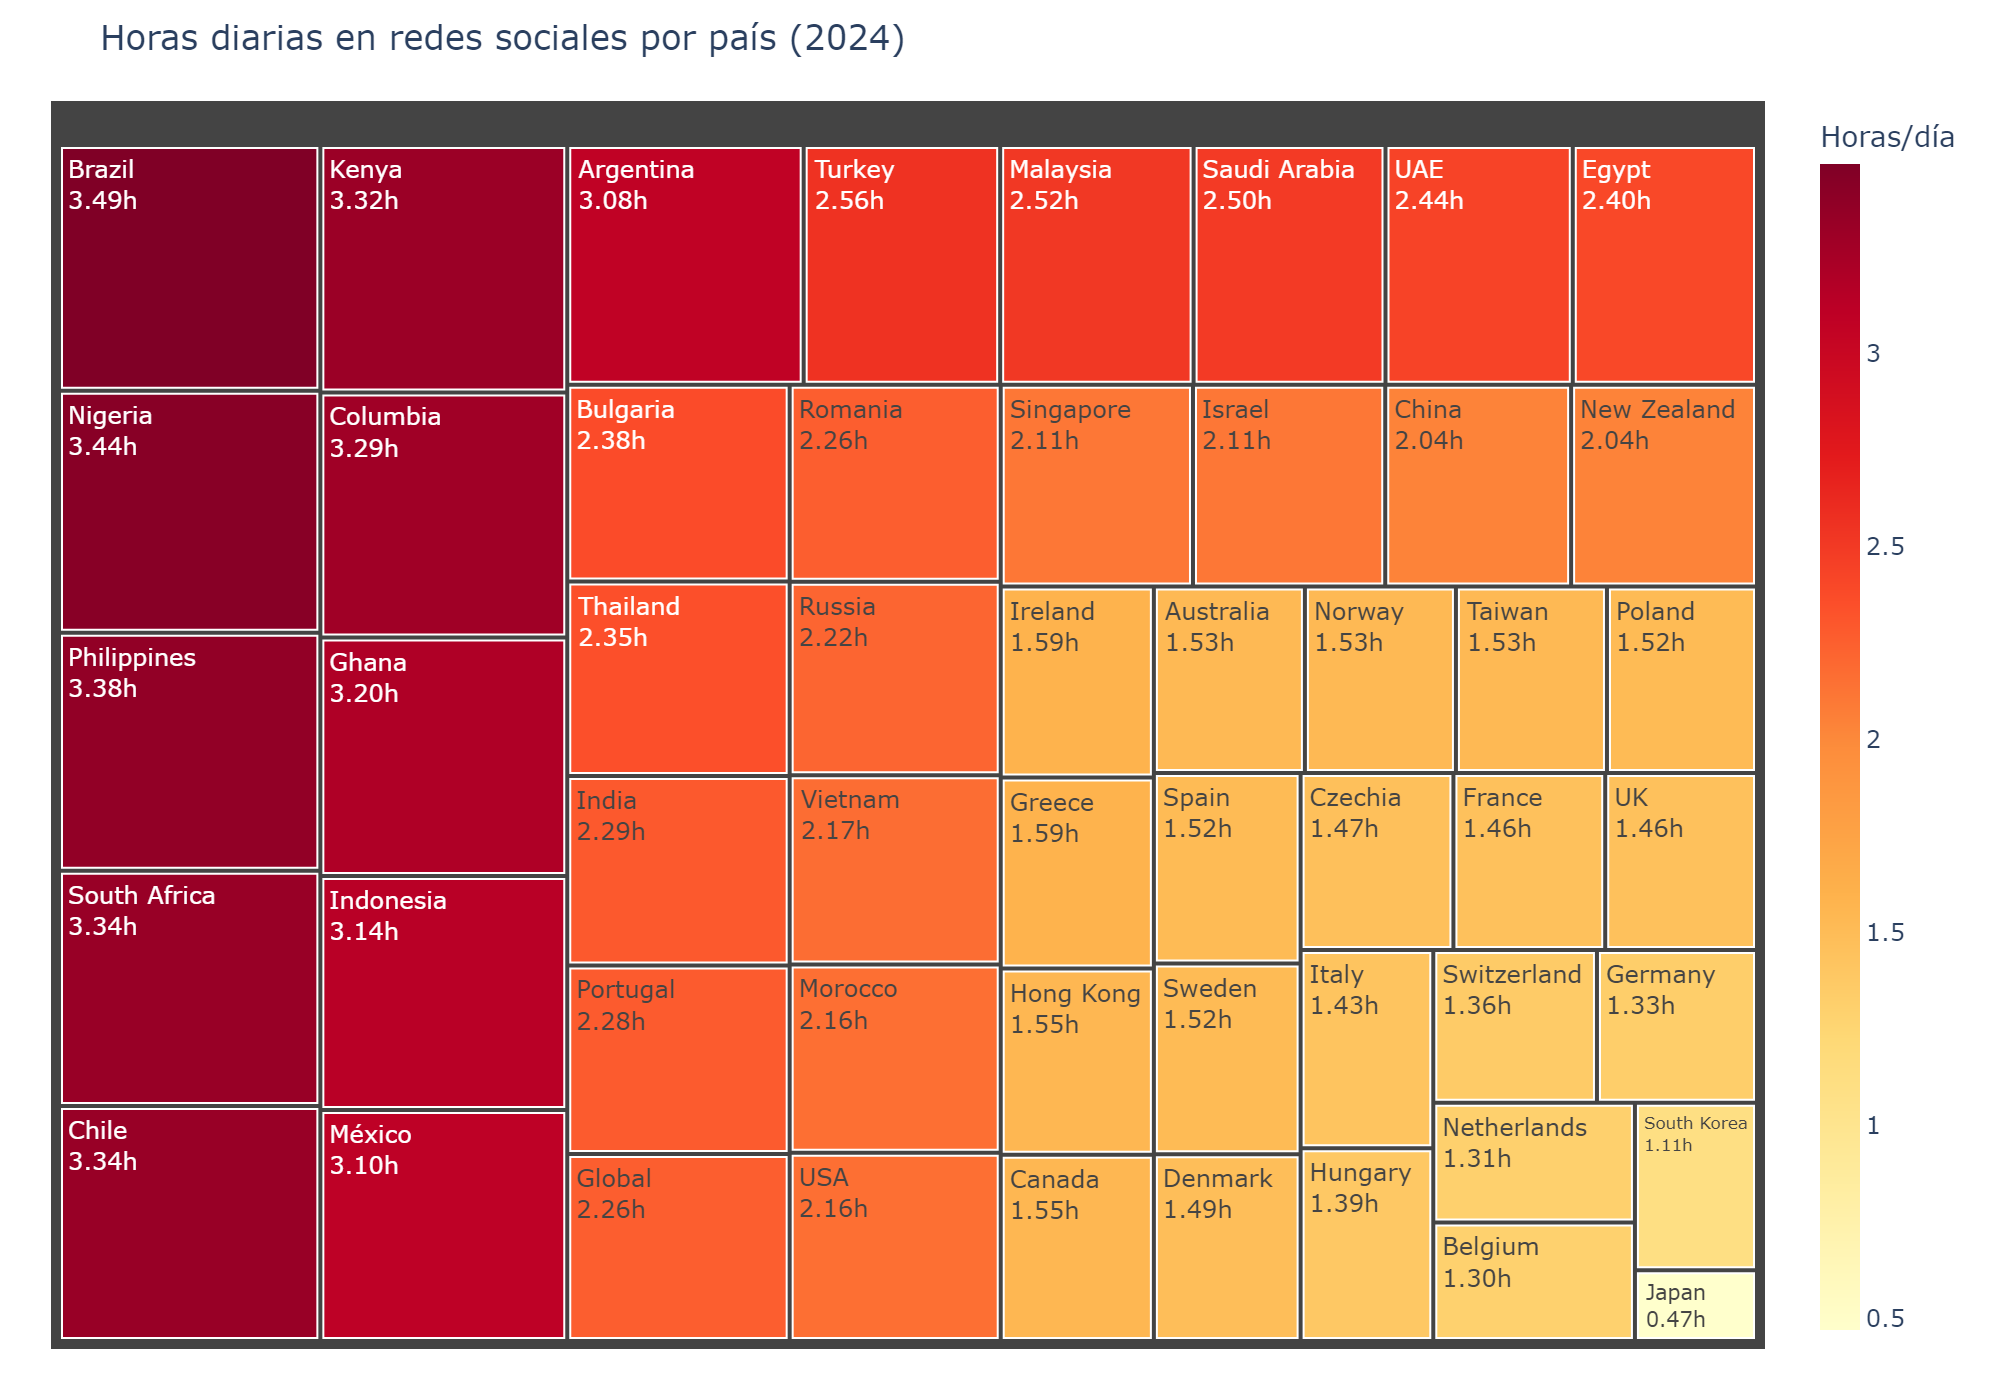
\includegraphics[width=0.85\textwidth]{images/graph1_JG.png}
    \caption{Fuente: Elaboración propia con datos de [Nombre de Fuente]}
\end{figure}

\subsubsection*{Conclusión}
Texto de conclusión específico para este gráfico. Analizar tendencias observadas y su relación con el impacto tecnológico en la vida cotidiana.

% Gráfico 2
\subsection*{Gráfico 2: Aquí colocar título}
\begin{figure}[H]
    \centering
    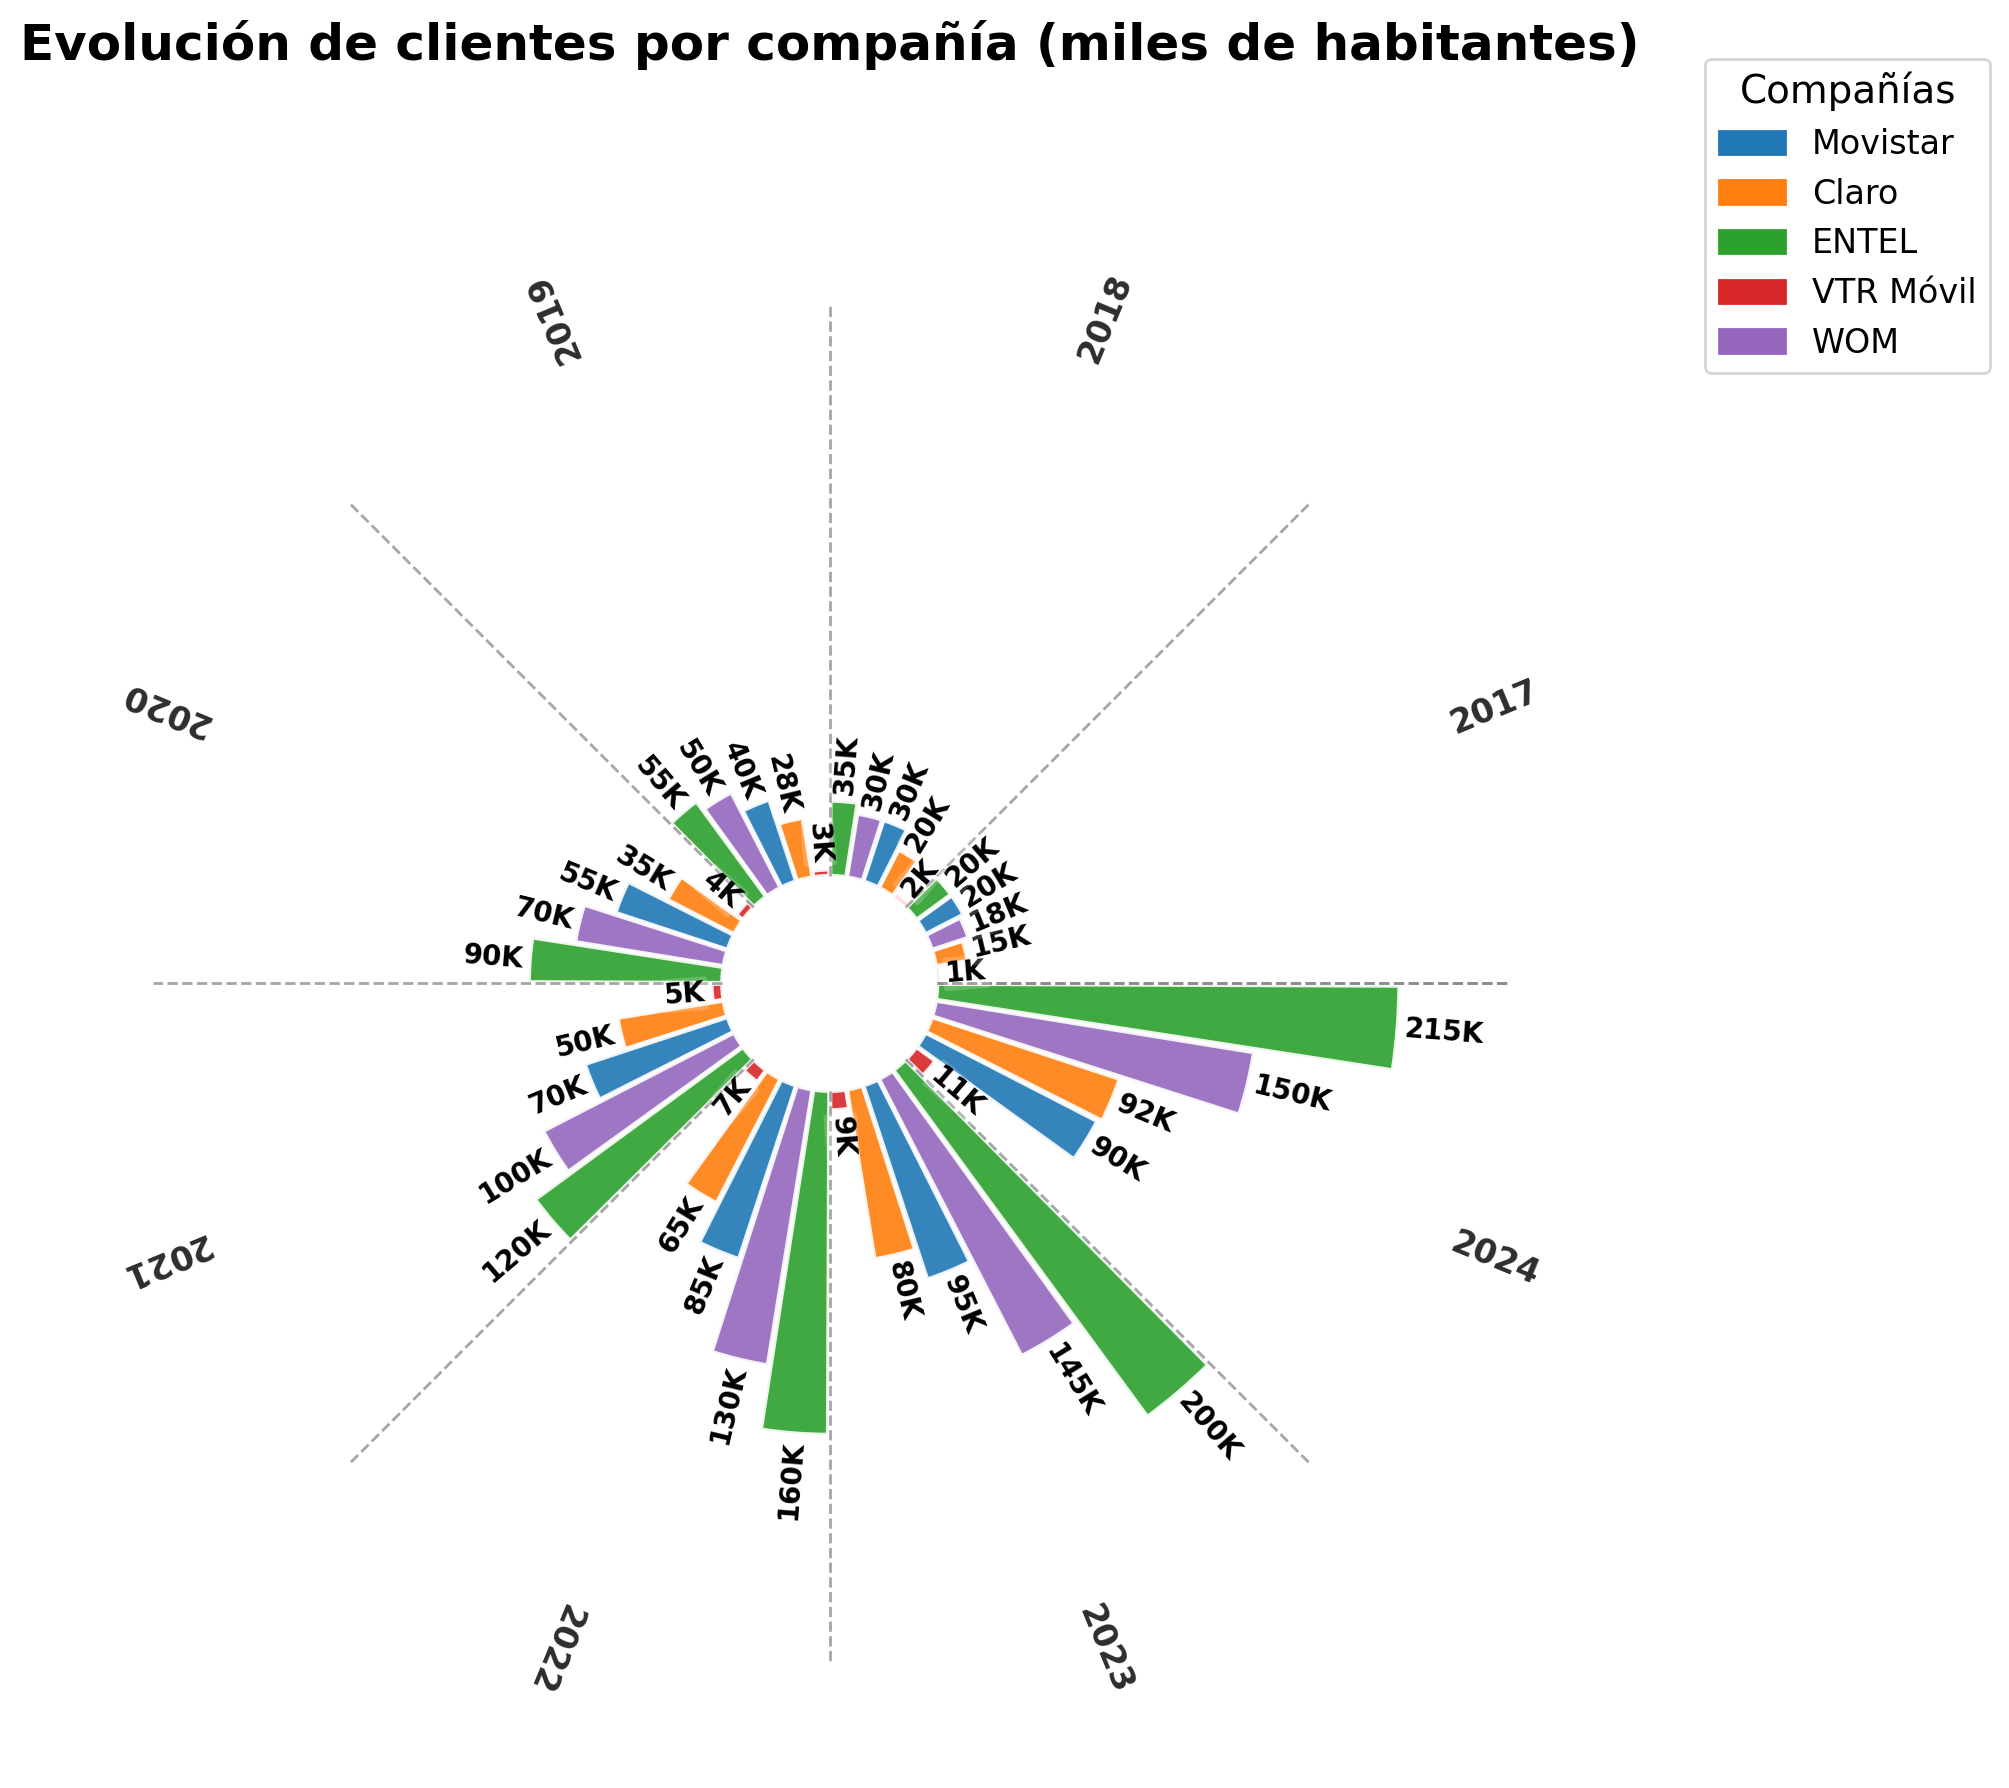
\includegraphics[width=0.85\textwidth]{images/graph2_JG.png}
    \caption{Fuente: Elaboración propia con datos de [Nombre de Fuente]}
\end{figure}

\subsubsection*{Conclusión}
Texto de conclusión específico para este gráfico. Analizar tendencias observadas y su relación con el impacto tecnológico en la vida cotidiana.

% Añadir los gráficos 3 al 6 siguiendo el mismo patrón

\section*{Conclusiones Generales}
\begin{itemize}
    \item Tendencia tecnológica dominante identificada
    \item Sector con mayor evolución tecnológica
    \item Impacto medible en la vida cotidiana
    \item Proyecciones futuras basadas en los datos
\end{itemize}

\end{document}